\documentclass[]{elsarticle} %review=doublespace preprint=single 5p=2 column
%%% Begin My package additions %%%%%%%%%%%%%%%%%%%
\usepackage[hyphens]{url}

  \journal{Journal of Transport Geography} % Sets Journal name


\usepackage{lineno} % add
\providecommand{\tightlist}{%
  \setlength{\itemsep}{0pt}\setlength{\parskip}{0pt}}

\usepackage{graphicx}
%%%%%%%%%%%%%%%% end my additions to header

\usepackage[T1]{fontenc}
\usepackage{lmodern}
\usepackage{amssymb,amsmath}
\usepackage{ifxetex,ifluatex}
\usepackage{fixltx2e} % provides \textsubscript
% use upquote if available, for straight quotes in verbatim environments
\IfFileExists{upquote.sty}{\usepackage{upquote}}{}
\ifnum 0\ifxetex 1\fi\ifluatex 1\fi=0 % if pdftex
  \usepackage[utf8]{inputenc}
\else % if luatex or xelatex
  \usepackage{fontspec}
  \ifxetex
    \usepackage{xltxtra,xunicode}
  \fi
  \defaultfontfeatures{Mapping=tex-text,Scale=MatchLowercase}
  \newcommand{\euro}{€}
\fi
% use microtype if available
\IfFileExists{microtype.sty}{\usepackage{microtype}}{}
\bibliographystyle{elsarticle-harv}
\ifxetex
  \usepackage[setpagesize=false, % page size defined by xetex
              unicode=false, % unicode breaks when used with xetex
              xetex]{hyperref}
\else
  \usepackage[unicode=true]{hyperref}
\fi
\hypersetup{breaklinks=true,
            bookmarks=true,
            pdfauthor={},
            pdftitle={Estimating spatial availability/mismatch using singly constrained accessibility measures},
            colorlinks=false,
            urlcolor=blue,
            linkcolor=magenta,
            pdfborder={0 0 0}}
\urlstyle{same}  % don't use monospace font for urls

\setcounter{secnumdepth}{0}
% Pandoc toggle for numbering sections (defaults to be off)
\setcounter{secnumdepth}{0}

% Pandoc citation processing
\newlength{\cslhangindent}
\setlength{\cslhangindent}{1.5em}
\newlength{\csllabelwidth}
\setlength{\csllabelwidth}{3em}
% for Pandoc 2.8 to 2.10.1
\newenvironment{cslreferences}%
  {}%
  {\par}
% For Pandoc 2.11+
\newenvironment{CSLReferences}[2] % #1 hanging-ident, #2 entry spacing
 {% don't indent paragraphs
  \setlength{\parindent}{0pt}
  % turn on hanging indent if param 1 is 1
  \ifodd #1 \everypar{\setlength{\hangindent}{\cslhangindent}}\ignorespaces\fi
  % set entry spacing
  \ifnum #2 > 0
  \setlength{\parskip}{#2\baselineskip}
  \fi
 }%
 {}
\usepackage{calc}
\newcommand{\CSLBlock}[1]{#1\hfill\break}
\newcommand{\CSLLeftMargin}[1]{\parbox[t]{\csllabelwidth}{#1}}
\newcommand{\CSLRightInline}[1]{\parbox[t]{\linewidth - \csllabelwidth}{#1}\break}
\newcommand{\CSLIndent}[1]{\hspace{\cslhangindent}#1}

% Pandoc header
\usepackage{booktabs}
\usepackage{longtable}
\usepackage{array}
\usepackage{multirow}
\usepackage{wrapfig}
\usepackage{float}
\usepackage{colortbl}
\usepackage{pdflscape}
\usepackage{tabu}
\usepackage{threeparttable}
\usepackage{threeparttablex}
\usepackage[normalem]{ulem}
\usepackage{makecell}
\usepackage{xcolor}



\begin{document}
\begin{frontmatter}

  \title{Estimating spatial availability/mismatch using singly
constrained accessibility measures}
    \author[Some School]{Author One}
   \ead{author.1@example.com} 
    \author[Some School]{Author Two\corref{Corresponding Author}}
   \ead{author.2@example.com} 
      \address[Some School]{Address}
      \cortext[1]{Corresponding Author}
  
  \begin{abstract}
  This is the abstract.

  It consists of two paragraphs.
  \end{abstract}
  
 \end{frontmatter}

\newpage

\hypertarget{introduction}{%
\section{Introduction}\label{introduction}}

The concept of accessibility is a relatively simple one whose appeal
derives from combining the spatial distribution of opportunities and the
cost of reaching them (Hansen, 1959). Numerous methods for calculating
accessibility have been proposed that can be broadly organized into
infrastructure-, place-, person-, and utility-based measures (Geurs and
van Wee, 2004). Of these, the place-based family of measures is arguably
the most common, capturing the number of opportunities reachable from an
origin using the transportation network. This type of measure is also
referred to as a gravity-based measure of accessibility that captures
the potential for interaction.

Accessibility analysis is widely employed in transportation, geography,
public health, and many other areas, and there is increasing emphasis on
a shift from mobility-oriented to accessibility-oriented planning
(Deboosere et al., 2018; Handy, 2020; Proffitt et al., 2017; Yan, 2021).
However, while these types of accessibility measures are excellent
indicators of the intersection between urban structure and
transportation infrastructure, they have been criticized in the past for
not being highly interpretable. Previous research has highlighted how
the weighting of opportunities using an impedance function can make
gravity measures more difficult for planners and policymakers to
interpret compared to simpler cumulative opportunity measures (Geurs and
van Wee, 2004; Miller, 2018). Moreover, because place-based
accessibility measures sensitive to the number of opportunities and the
characteristics of the transportation network, raw accessibility values
cannot be easily compared across study areas (Allen and Farber, 2019).

It is also unclear what the highest and lowest levels of accessibility
in the region actually represent. The ``total accessibility'' in the
region is not a meaningful quantity since it is not constrained to
resemble, let alone match the number of opportunities available in a
region. Furthermore, while accessibility depends on the supply of
destination opportunities weighted by the travel costs associated with
reaching them, the calculated accessibilities are not sensitive to the
demand for those opportunities at the origins. Put another way,
traditional measures of place-based accessibility do not capture the
competition for opportunities. This theoretical shortcoming (Geurs and
van Wee, 2004) is particularly problematic when those opportunities are
``non-divisible'' in the sense that, once they have been taken by
someone, are no longer available to other members of the population.
Examples of indivisible opportunities include jobs (when a person takes
up a job, the same job cannot be taken by someone else) and seats at
schools (once a student takes a seat at a school, that particular
opportunity is no longer there for another student). From a different
perspective, employers may see workers as opportunities, so when a
worker takes a job, this particular individual is no longer in the
available pool of candidates for hiring.

To remedy these issues, researchers have proposed several different
approaches for calculating competitive accessibility measures. On the
one hand, this includes several approaches that first normalize the
number of opportunities available at a destination by the demand for
them from the origin zones and, second, sum the demand-corrected
opportunities reachable from the origins (e.g. Joseph and Bantock
(1984); Shen (1998)). These advances were popularized in the family of
two-step floating catchment area methods (Luo and Wang, 2003) that have
found widespread adoption for calculating competitive accessibility to
healthcare and other uses. However, while floating catchment areas
purport to account for competition/congestion effects, but as discussed
by Paez, Higgins, and Vivona (2019), they are vulnerable to
inflation/deflation issues due to the multiple counting of demand and
supply, which makes them prone to bias unless corrected.

A second approach is to impose constraints on the gravity model to
ensure flows between zones are equal to the observed totals. Based on
Wilson's (1971) spatial interaction models, researchers can incorporate
a single or pair of constraints that control the magnitude of flows from
zone \(i\) to \(j\) are equal to the demand at \(i\) and the number of
opportunities at \(j\). Allen and Farber (2019) recently incorporated a
version of the doubly-constrained gravity model within the floating
catchment area approach to calculate competitive accessibility to
accessibility using transit across eight cities in Canada. But while
such a model can account for competition, the mutual dependence of the
balancing factors in a doubly-constrained model means they must be
iteratively calculated and thus more computationally-intensive.

As an alternative to place-based measures of competitive accessibility,
we propose a measure of \emph{spatial availability} to capture the
number of indivisible opportunities that are realistically available to
the opportunity-seeking population. As we will show, spatial
availability is a singly-constrained measure of accessibility.
By\ldots{} this method avoids the issues of inflation that result from
multiple counting of opportunities in traditional accessibility
measures. The method returns meaningful accessibilities that correspond
to the rate of available opportunities per person. Moreover, the method
also returns a benchmark value for the region under study against which
results for individual origins can be compared.

In the following sections we will describe and illustrate this new
measure using simple numerical examples. First, we will describe the
measure. Second, we will calculate the spatial availability of jobs from
the perspective of the population. Then, we will calculate the spatial
availability of workers from the perspective of employers. Next, we will
illustrate how to calculate the spatial availability with catchment
restrictions. Finally, we will compare conventional accessibility
estimates to the proposed measure of spatial availability.

\hypertarget{background}{%
\section{Background}\label{background}}

Most accessibility measures (excluding utility-based measures) are
derived from the gravity model, and are known as \emph{gravity-based}
accessibility. Briefly, consider the following conventional
accessibility measure \(A_i\) :

\[
A_i = \sum_{j=1}^JO_jf(c_{ij})
\]

\noindent where:

\begin{itemize}
\tightlist
\item
  \(i\) is a set of origin locations.
\item
  \(j\) is a set of destination locations.
\item
  \(O_j\) is the number of opportunities at location \(j\). These are
  opportunities for activity and add some sort of \emph{supply} to the
  area;
\item
  \(c_{ij}\) is a measure of the cost of moving between \(i\) and \(j\)
\item
  \(f(\cdot)\) is an impedance (or distance-decay) function (a
  monotonically non-increasing or decreasing function of \(c_{ij}\)).
\end{itemize}

The accessibility value \(A_i\), it can be seen, is the weighted sum of
opportunities that can be reached from location \(i\), given the cost of
travel \(c_{ij}\) and an impedance function. Summing the opportunities
in the neighborhood of \(i\) (the neighborhood is defined by the
impedance function) estimates of the total number of opportunities that
can be reached from \(i\) at a certain cost. Depending on the impedance
function, the measure could be cumulative opportunities (if \(f(\cdot)\)
is a binary or indicator function) or a more traditional gravity
measure, for instance with a Gaussian impedance function or an inverse
cost impedance function.

We use a simple numerical example to introduce the key concepts, and we
will use the usual accessibility measure for comparison. In this way, we
aim to show the differences between accessibility and spatial
availability, which helps to explain how spatial availability can
improve interpretability in the analysis of spatially dispersed
opportunities.

\hypertarget{numerical-example}{%
\subsection{Numerical Example}\label{numerical-example}}

In this section we present a simple numerical example. The setup for the
example is a system with three employment centers and nine population
centers, as seen in Table \ref{tab:toy-example}.

\begin{table}

\caption{\label{tab:toy-example-table}\label{tab:toy-example}Numerical example}
\centering
\resizebox{\linewidth}{!}{
\begin{tabular}[t]{lrl>{}l}
\toprule
id & number & type & \\
\midrule
E1 & 750 & jobs & \\

E2 & 2250 & jobs & \\

E3 & 1500 & jobs & \\

P1 & 260 & population & \\

P2 & 255 & population & \\

P3 & 510 & population & \\

P4 & 495 & population & \\

P5 & 1020 & population & \\

P6 & 490 & population & \\

P7 & 980 & population & \\

P8 & 260 & population & \\

P9 & 255 & population & \multirow{-12}{*}{\raggedright\arraybackslash 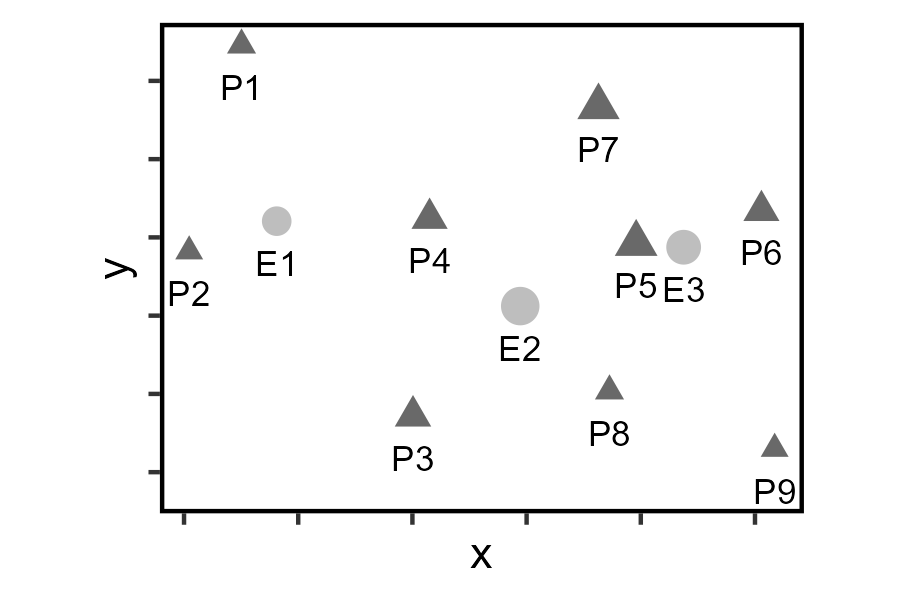
\includegraphics{images/figure-1.png}}\\
\bottomrule
\end{tabular}}
\end{table}

The accessibility to employment of each of the population centers can be
calculated using the expression above for \(A_i\). As noted, this yields
the number of jobs (opportunities) that are accessible (i.e., can be
reached) from each population center, given the cost. In this example we
use the straight line distance between the population and jobs for
\(c_{ij}\), and a negative exponential function with \(\beta = 0.0015\).

\begin{figure}
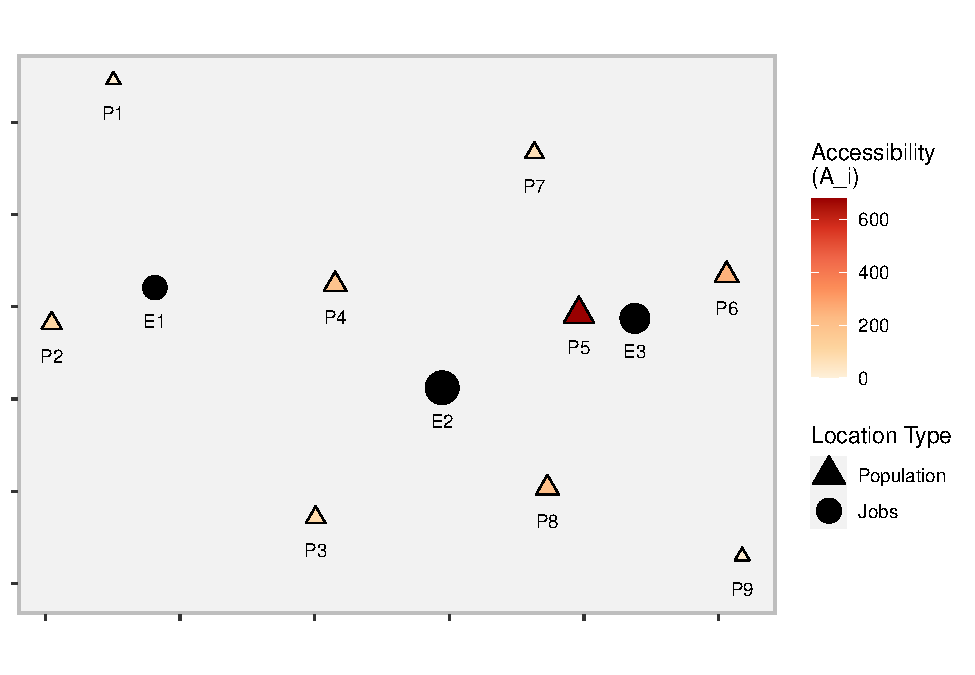
\includegraphics[width=1\linewidth]{Spatial-Availability_files/figure-latex/toy-example-accessibility-plot-1} \caption{\label{fig:toy-example-accessibility}Accessibility results using simple numerical example}\label{fig:toy-example-accessibility-plot}
\end{figure}

Figure \ref{fig:toy-example-accessibility} shows the three employment
centers (black circles), with the size of the symbol in proportion to
the number of jobs there. We also see nine population centers
(triangles), where the size of the symbol is proportional to the
accessibility to jobs. At a quick glance:

\begin{itemize}
\item
  Population centers (triangles) in the middle of the map are relatively
  close to all three employment centers and thus have the highest levels
  of job accessibility. Population center P5 is relatively central and
  close to all employment centers, and it is the closest population to
  the second largest employment center in the region. Unsurprisingly,
  this population center has the highest accessibility 680.64);
\item
  Population centers (triangles) near the left edge of the map (only in
  proximity to the small employment center) have the lowest levels of
  job accessibility. Population center P1 is quite peripheral and the
  closest emplyment center is also the smallest one. Concequently, it
  has the lowest accessibility with \(A_i=\) 17.12);
\end{itemize}

\hypertarget{what-are-the-issues}{%
\subsection{What are the Issues?}\label{what-are-the-issues}}

Accessibility measures such as that illustrated above are excellent
indicators of the intersection between urban structure and
transportation infrastructure. However, beyond enabling comparisons of
cardinality (e.g., P5 has higher accessibility than P1, which although
low is still better than zero) they are not highly interpretable on
their own. First, total accessibility \(\sum_{i=1}^IA_i\), if
calculated, depends on the number of origins: since every additional
origin in the analysis makes at least one and possibly more
opportunities at destinations to be multiple-counted, total
accessibility does not match the total number of opportunities available
in the study area. Moreover, this property means total accessibility is
vulnerable to the modifiable areal unit problem.

Second, the calculated accessibilities do not take competition into
account. For example, an individual at P5 in the example has
accessibility to 680.6373657 jobs. But since this is also a large
population center, there is potentially large competition for those
accessible jobs. In other words, the value of \(A_i\) is not sensitive
to the size of population at the origin seeking the opportunity (in this
case jobs), let alone the population at other locations. This
unfortunately limits the interpretability of the measure. Floating
catchment areas purport to account for competition/congestion effects,
but as discussed by Paez, Higgins, and Vivona (2019), they are
vulnerable to inflation/deflation issues, which makes them prone to bias
unless corrected. As an alternative, we propose a singly-constrained
gravity measure that corresponds to the concept of \emph{spatial
availability} or \emph{mismatch}.

\hypertarget{spatial-availabilitymismatch}{%
\section{Spatial
Availability/Mismatch}\label{spatial-availabilitymismatch}}

\hypertarget{definitions}{%
\subsection{Definitions}\label{definitions}}

As recent research on accessibility shows (see for instance Paez,
Higgins, Vivona (2019) and Allen and Farber (2019)), accounting for
competitive access in a meaningful way requires the proportional
allocations of quantities in the accessibility calculations, or their
normalization. At issue is the fact that multiple-counting is
commonplace when calculating conventional accessibility \(A_i\) for
\(i=1,\cdots,n\). This is easy to see once we realize that every
opportunity enters the weighted sum once for every origin \(i\) that can
reach it. This has the unfortunate effect of obscuring the
interpretability of \(A_i\) and fails to answer for a individual at a
specific population center the question: ``many jobs are accessible, but
the same jobs are also accessible to my (possibly) numerous
neighbors\ldots what does high accessibility actually mean to me?''

In the spatial availability framework proposed, and in line with the
gravity tradition, we distinguish between opportunities at a destination
and demand for opportunities at the origin. To explain the analytical
framework, the example of accessibility to employment is illustrative,
with ``population'' in the role of demand and ``jobs'' in the role of
opportunities.

We begin with allocation based on demand (the number of individuals in
the population in the labor market who ``demand'' employment). Consider
an employment center \(j\) with \(O_j^r\) jobs of type \(r\). In the
general case where there are \(K\) population centers in the region, the
following factor can be defined to allocate the jobs proportionally
based on the size of the population at each center:

\[
f^p_{ij} = \frac{P_{i\in r}^\alpha}{\sum_{k=1}^K P_{k\in r}^\alpha}
\]

\noindent where \(f^p_{ij}\) is a factor that proportionally allocates a
share of the jobs at \(j\) to population center \(i\). On the right hand
side of the equation, \(P_{k\in r}\) is the population at location \(k\)
that is eligible for jobs of type \(r\) (maybe those with a certain
level of training, or in a designated age group). Here we add an
empirical parameter \(\alpha\) that can be used to modulate the effect
of size in the calculations (i.e., if \(\alpha <1\) employment centers
draw more rapidly from small centers than from large centers, and when
\(\alpha>1\) employment centers draw more rapidly from large population
centers). The summation in the bottom is over \(k=1,\cdots,K\), the
number of population centers in the region. The factors \(f_{kj}^p\)
satisfy the property that \(\sum_k^{K} f^p_{kj} = 1\).

The share of jobs at \(j\) allocated to (i.e., available to) each
population center is:

\[
V_{kj} = W_jf^p_{kj}
\]

\noindent and since \(\sum_k^{K} f^p_{kj} = 1\) it follows that:

\[
\sum_{k=1}^K V_{kj} = W_j 
\]

In other words, the number of jobs is preserved.

As an example, consider an employment center \(j\) in a region with two
population centers (say \(i\) and \(k\)). For simplicity, assume that
the all the population in the region is eligible for these jobs, that
is, that the entirety of the population is included in the set \(r\).
The allocation factors for the jobs at \(j\) would be:

\[
\begin{array}{l}\
f^p_{ij} = \frac{P_i ^\alpha}{P_i^\alpha + P_k^\alpha}\\
f^p_{kj} = \frac{P_k^\alpha}{P_i^\alpha + P_k^\alpha}\\
\end{array}
\]

Suppose that there are three hundred jobs in the employment center
(\(W_j = 300\)), and that the populations are \(P_j=240\) and
\(P_k=120\). The jobs are allocated as follows (assuming that
\(\alpha=1\)):

\[
\begin{array}{l}\
V_{ij} = W_j\frac{P_i^\alpha}{P_i^\alpha + P_k^\alpha} = 300\frac{240}{240 + 120} = 300\frac{240}{360} = 200\\
V_{kj} = W_j\frac{P_k^\alpha}{P_i^\alpha + P_k^\alpha} = 300\frac{120}{240 + 120} = 300\frac{120}{360} = 100 \\
\end{array}
\]

It can be seen that proportionally more jobs are allocated to the bigger
center and also that the total number of jobs is preserved
(\(\sum_{k=1}^K W_{kj} = W_j\)).

The factors above account for the total number of opportunities at the
destination (i.e., the number of jobs at the employment center), but
they do not account for their location relative to the population
centers. The proportional allocation procedure above is insensitive to
how far population center \(i\) is from employment center \(j\). To
account for this effect we define a second set of allocation factors
based on distance to the employment centers. These are defined as: \[
f^c_{ij} = \frac{f(c_{ij})}{\sum_{k=1}^K f(c_{kj})}
\]

\noindent where \(c_{ij}\) is the cost (e.g., the distance, travel time,
etc.) to employment center \(j\) from population center \(i\), and
\(f(\cdot)\) is an impedance function, that is a monotonically
decreasing function of \(c_{kj}\). The idea is that proportionally more
jobs are allocated to closer locations. Assume that the impedance
function is a negative exponential function as follows, and assume that
\(\beta\) (which modulates the steepness of the impedance effect and is
an empirical parameter) is one:

\[
f(c_{ij}) = \exp(-\beta c_{ij})
\]

Continuing the example, suppose that the distance from population center
\(i\) to employment center \(j\) is 0.6 km, and the distance from
population center \(k\) to employment center \(j\) is 0.3 km. Being
closer, we would expect more jobs to be allocated to the population of
\(i\). The jobs would be sorted as follows:

\[
\begin{array}{l}\
f^c_{ij} = \frac{\exp(-\beta D_{ij})}{\exp(-\beta D_{ij}) + \exp(-\beta D_{kj})}\\
f^c_{kj} = \frac{\exp(-\beta D_{kj})}{\exp(-\beta D_{ij}) + \exp(-\beta D_{kj})}\\
\end{array}
\]

Numerically, the jobs allocation is:

\[
\begin{array}{l}\
V^d_{ij} = W_j\frac{\exp(-D_{ij})}{\exp(-D_{ij}) + \exp(-D_{kj})} = 300\frac{\exp(-0.6)}{\exp(-0.6) + \exp(-0.3)} = 3\times 0.426 = 127.8\\
V^d_{kj} = W_j\frac{\exp(-D_{kj})}{\exp(-D_{ij}) + \exp(-D_{kj})} = 300\frac{\exp(-0.3)}{\exp(-0.6) + \exp(-0.3)} = 3\times  0.574 = 172.2\\
\end{array}
\]

A larger share of jobs is allocated to the population center that is
closest. As before, the sum of jobs allocated to the population centers
matches the total number of jobs available.

We can combine the proportional allocation factors by population and
distance as follows:

\[
V_{ij} = W_i\frac{f^p_{ij} \cdot f^c_{ij}}{\sum_{k=1}^K f^p_{kj} \cdot f^c_{kj}}
\]

In the example:

\[
\begin{array}{l}\
V_{ij} = W_j\cdot \frac{f^o_{ij} \cdot f^c_{ij}}{f^o_{ij} \cdot f^c_{ij} + f^o_{kj} \cdot f^c_{kj}} = 300 \frac{\big(\frac{2}{3} \big) \big(0.426 \big)}{\big(\frac{2}{3} \big) \big(0.426 \big) + \big(\frac{1}{3} \big) \big(0.574 \big)} = \big(300 \big)\big(\frac{0.284}{0.475} \big)= 179.4\\
V_{kj} = W_j\cdot \frac{f^o_{kj} \cdot f^c_{kj}}{f^o_{ij} \cdot f^c_{ij} + f^o_{ik} \cdot f^c_{ik}} = 300 \frac{\big(\frac{1}{3} \big) \big(0.574 \big)}{\big(\frac{2}{3} \big) \big(0.426 \big) + \big(\frac{1}{3} \big) \big(0.574 \big)}  = \big(300 \big)\big(\frac{0.191}{0.475} \big)= 120.6 \\
\end{array}
\]

Notice how fewer jobs are allocated to population center \(i\) compared
to the allocation by population only, to account for the higher cost of
reaching the employment center. On the other hand, distance alone
allocated more jobs to the closest population center (i.e., \(k\)), but
since it is smaller, it also get a smaller share of the jobs overall.
Again, the sum of jobs at employment center \(j\) that are allocated to
population centers \(i\) and \(k\) simultaneously based on
\emph{population-} and \emph{distance-} based allocation is preserved
(i.e., \(W_{ij} + W_{kj} = W_j\)).

Availability is simply the sum of the above by origin:

\[
V_i = \sum_{j=1}^J V_{ij}
\]

This quantity represents opportunities (e.g., jobs) that can be reached
from \(i\) (i.e., they are accessible), and that are \emph{not}
allocated to a competitor: therefore the weighted sum of available
opportunities. Compare \(V_i\) to the singly-constrained gravity model
(see Wilson \href{https://doi.org/10.1068/a030001}{(1971)}). In essence,
\(V_i\) is the result of constraining \(A_i\) to match one of the
marginals in the origin-destination table, the known total of
opportunities.

Since the sum of opportunities is preserved in the procedures above, it
is possible to calculate a highly interpretable measure of spatial
availability per capita (call it lower-case \(v_i\)) as follows:

\[
v_i = \frac{V_i}{P_i}
\]

In the example above:

\[
\begin{array}{l}\
v_{ij} = \frac{V_{ij}}{P_i} =  \frac{179.4}{240}\\
v_{kj} =  \frac{V_{ik}}{P_k} =  \frac{120.6}{120}\\
\end{array}
\]

Less competition (\(P_k\) is the smallest population center in the
region) and being closer to the jobs clearly works in favor of
individuals at \(k\). Where the overall ratio of jobs to population in
the region is \(300/(240 + 120)=\) 0.83, the spatially available jobs
per capita at \(k\) is closer to unity.

In the following sections we use the same numerical example presented
above to illustrate how availability \(V_i\) is calculated. We conclude
by contrasting the two measures in the final section.

\hypertarget{st-use-case-available-jobs-for-the-working-population}{%
\subsection{1st Use Case: Available Jobs for The Working
Population}\label{st-use-case-available-jobs-for-the-working-population}}

In the following examples we use the same impedance function that was
used to illustrate the accessibility calculations in the numerical
example. The spatial availability calculations are implemented in the
function \texttt{sp\_avail}. The inputs are an Origin-Destination table
with labels for the origins (\texttt{o\_id}), labels for the
destinations (\texttt{d\_id}), the population (\texttt{pop)} and number
of opportunities (\texttt{opp}), an indicator for catchments or other
eligibility constraints (\texttt{r}), and a pre-calculated impedance
function (\texttt{f}). For this example, we assume that there are no
catchment restrictions by setting \texttt{r} to 1.

The value of the function (its output) is a vector with \(V_ij\) given
the inputs, that is, the opportunities available to \(i\) from \(j\):

\begin{verbatim}
[1] 4500
\end{verbatim}

\begin{verbatim}
[1] 4500
\end{verbatim}

\begin{verbatim}
# A tibble: 9 x 2
  Origin          V_i
  <fct>         <dbl>
1 Population 1   67.0
2 Population 2  414. 
3 Population 3  336. 
4 Population 4  745. 
5 Population 5 2081. 
6 Population 6  270. 
7 Population 7  256. 
8 Population 8  316. 
9 Population 9   14.9
\end{verbatim}

The following plot shows the estimates of spatial availability:

\begin{figure}
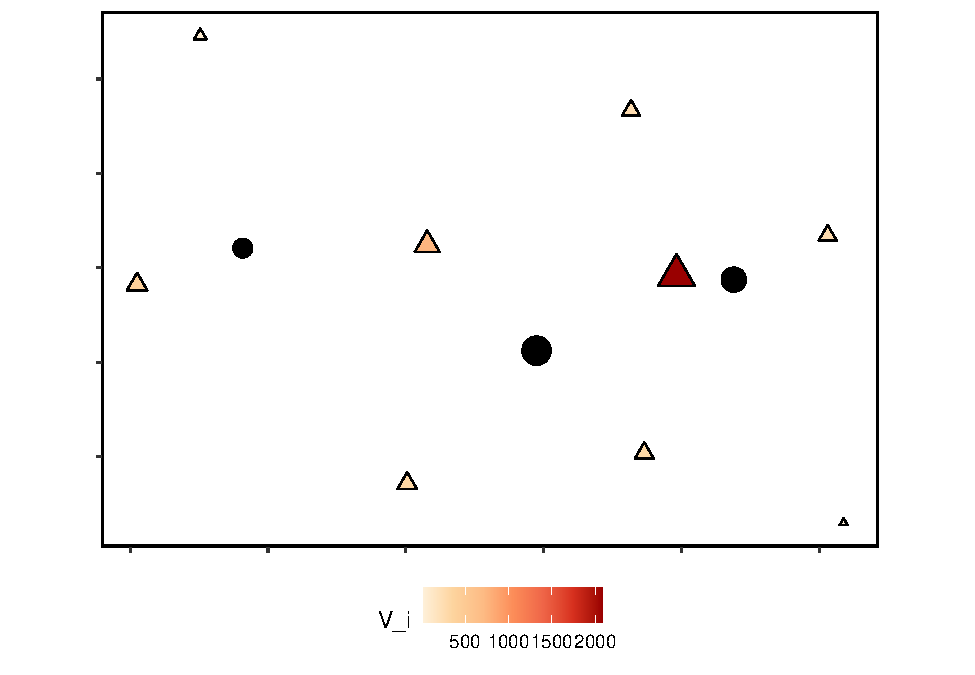
\includegraphics[width=1\linewidth]{Spatial-Availability_files/figure-latex/toy-example-availability-jobs-1} \caption{\label{fig:toy-example-availability-jobs}Spatial availability of jobs}\label{fig:toy-example-availability-jobs}
\end{figure}

We see that population center 5 has the highest level of spatial
availability, due to being a large population center that is moreover
relatively close to jobs. To improve the interpretability of this
measure, we first note that the regional measure of jobs per capita is
0.994. We then calculate the spatially available jobs per person at each
population center:

\begin{verbatim}
            id        v_i
1 Population 1 0.25787932
2 Population 2 1.62445872
3 Population 3 0.65947335
4 Population 4 1.50495734
5 Population 5 2.03989862
6 Population 6 0.55082935
7 Population 7 0.26164373
8 Population 8 1.21352615
9 Population 9 0.05842544
\end{verbatim}

Plot the spatial availability per person:

\begin{figure}
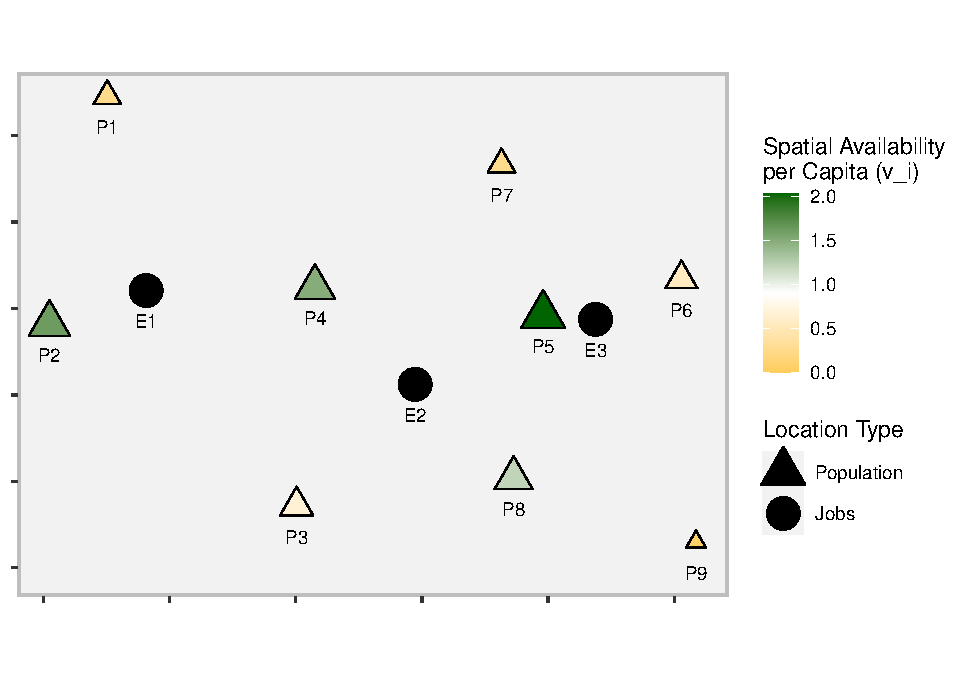
\includegraphics[width=1\linewidth]{Spatial-Availability_files/figure-latex/toy-example-availability-jobs-per-capita-1} \caption{\label{fig:toy-example-availability-jobs-per-capita}Spatial availability of jobs per capita}\label{fig:toy-example-availability-jobs-per-capita}
\end{figure}

Some population centers have almost two jobs available per person
(compared to the overall regional value of approximately one job per
capita), while others have less than one job available per person. This
does not mean that people are not taking some of the jobs. It means that
controlling for the cost of reaching jobs, they are worse off than those
with more jobs spatially available.

\hypertarget{nd-use-case-available-workers-for-employment-centers}{%
\subsection{2nd Use Case: Available Workers for Employment
Centers}\label{nd-use-case-available-workers-for-employment-centers}}

We can also examine the pool of workers available to each employment
center by considering the workers as the opportunities and the jobs as
the population.

Calculate the proportional allocation of jobs to population (referred to
as \(W_ji\)):

\begin{verbatim}
[1] 4525
\end{verbatim}

\begin{verbatim}
[1] 4525
\end{verbatim}

\begin{verbatim}
# A tibble: 3 x 2
  Destination           W_j
  <fct>               <dbl>
1 Employment Center 1  610.
2 Employment Center 2 1710.
3 Employment Center 3 2205.
\end{verbatim}

Plot the availability estimates:

\begin{figure}
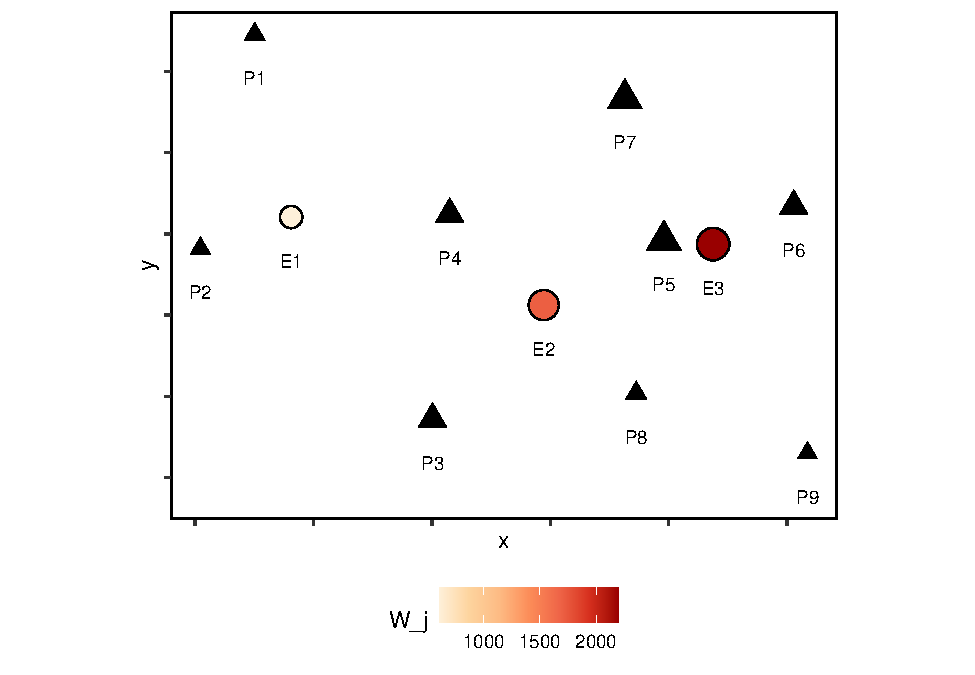
\includegraphics[width=1\linewidth]{Spatial-Availability_files/figure-latex/toy-example-availability-workers-1} \caption{\label{fig:toy-example-availability-workers}Spatial availability of workers}\label{fig:toy-example-availability-workers}
\end{figure}

\begin{verbatim}
                   id       w_j
1 Employment Center 1 0.8137264
2 Employment Center 2 0.7597858
3 Employment Center 3 1.4701247
\end{verbatim}

Plot the spatial availability of workers per job:

\begin{figure}
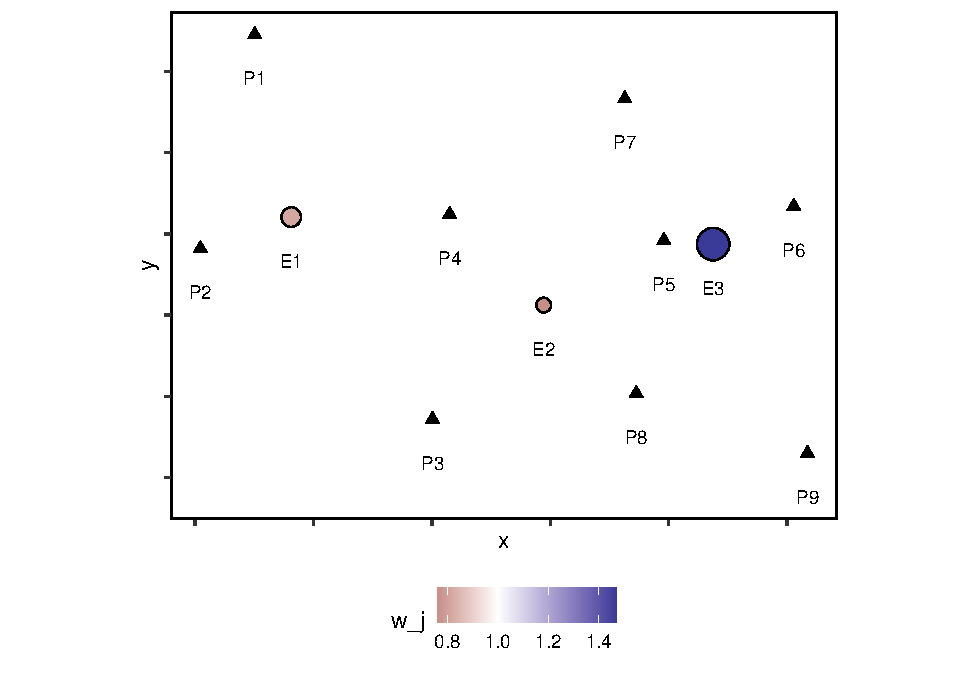
\includegraphics[width=1\linewidth]{Spatial-Availability_files/figure-latex/toy-example-availability-workers-per-job-1} \caption{\label{fig:toy-example-availability-workers-per-job}Spatial availability of workers per job}\label{fig:toy-example-availability-workers-per-job}
\end{figure}

\hypertarget{rd-use-case-available-jobs-for-specialized-working-populations}{%
\subsection{3rd Use Case: Available Jobs for Specialized Working
Populations}\label{rd-use-case-available-jobs-for-specialized-working-populations}}

In this section we introduce catchment/eligibility constraints. Due to
differences in educational achievement among the population, the jobs in
Employment Center 1 can only be taken by individuals in population
centers 1 and 2. Jobs in Employment Center 2 can be taken by individuals
in population centers 3, 4, 5, 7, and 8. Lastly, jobs in Employment
Center 3 require qualifications available only among individuals in
population centers 5, 6, 8, and 9. See figure below.

\begin{figure}
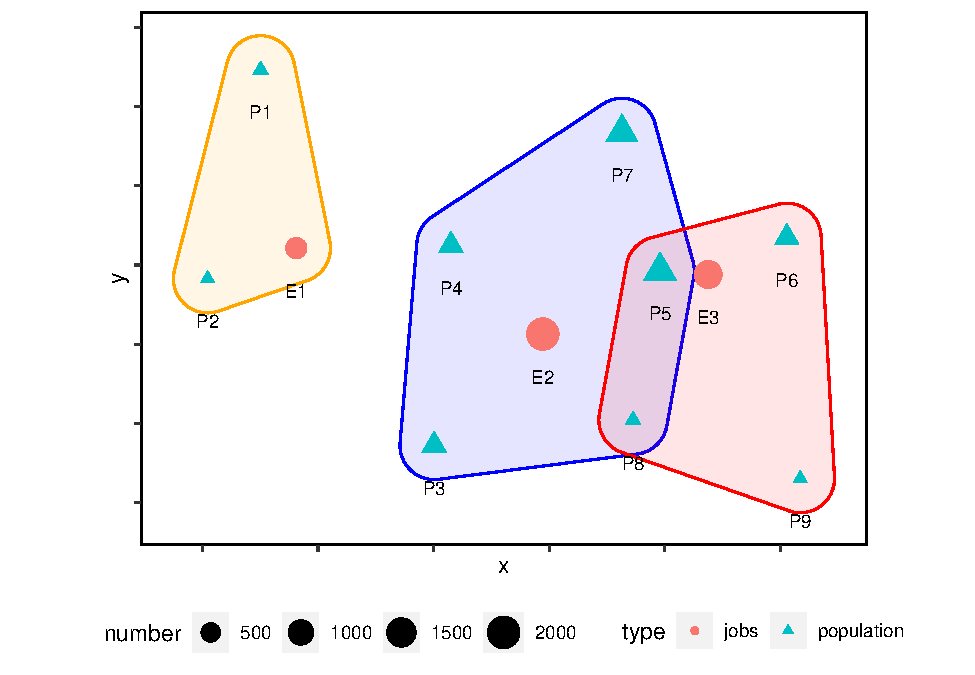
\includegraphics[width=1\linewidth]{Spatial-Availability_files/figure-latex/toy-example-plot-catchments-1} \caption{\label{fig:toy-example-catchments}Catchments areas in numeric example}\label{fig:toy-example-plot-catchments}
\end{figure}

\begin{verbatim}
[1] 4500
\end{verbatim}

\begin{verbatim}
[1] 4500
\end{verbatim}

\begin{verbatim}
# A tibble: 9 x 2
  Origin         V_i_r
  <fct>          <dbl>
1 Population 1  104.  
2 Population 2  646.  
3 Population 3  303.  
4 Population 4  527.  
5 Population 5 2173.  
6 Population 6  257.  
7 Population 7  161.  
8 Population 8  322.  
9 Population 9    7.52
\end{verbatim}

Plot the availability estimates:

\begin{figure}
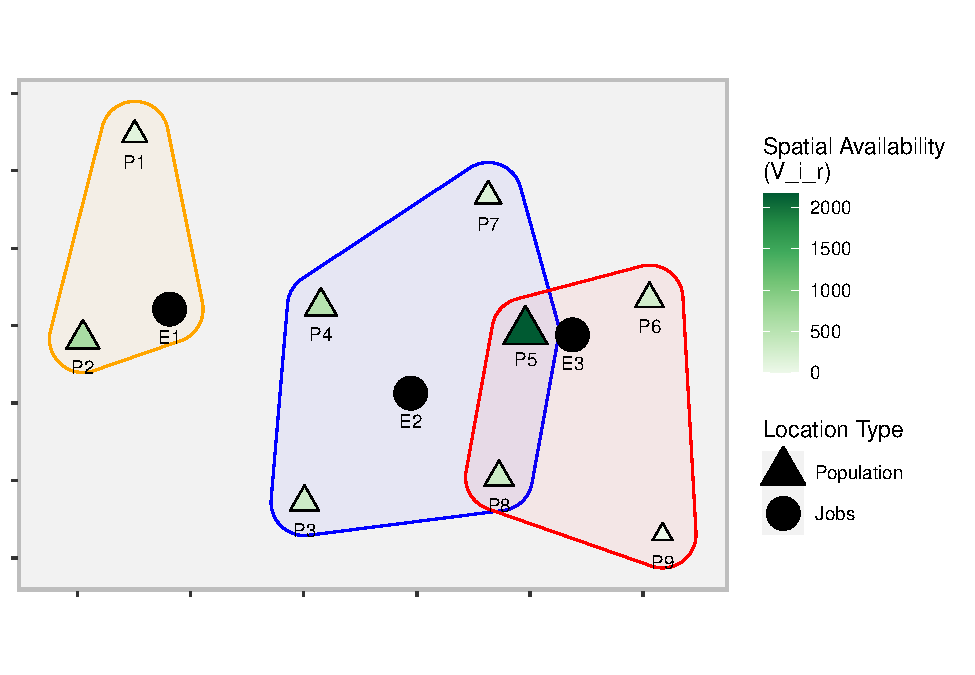
\includegraphics[width=1\linewidth]{Spatial-Availability_files/figure-latex/toy-example-availability-with-catchments-1} \caption{\label{fig:toy-example-availability-with-catchments}Spatial availability of jobs with catchment restrictions}\label{fig:toy-example-availability-with-catchments}
\end{figure}

Available jobs per person with catchment/eligibility conditions:

The plot in Fig.
\ref{fig:toy-example-availability-with-catchments-per-capita} shows the
availability per person without and with catchment restrictions.

\begin{figure}
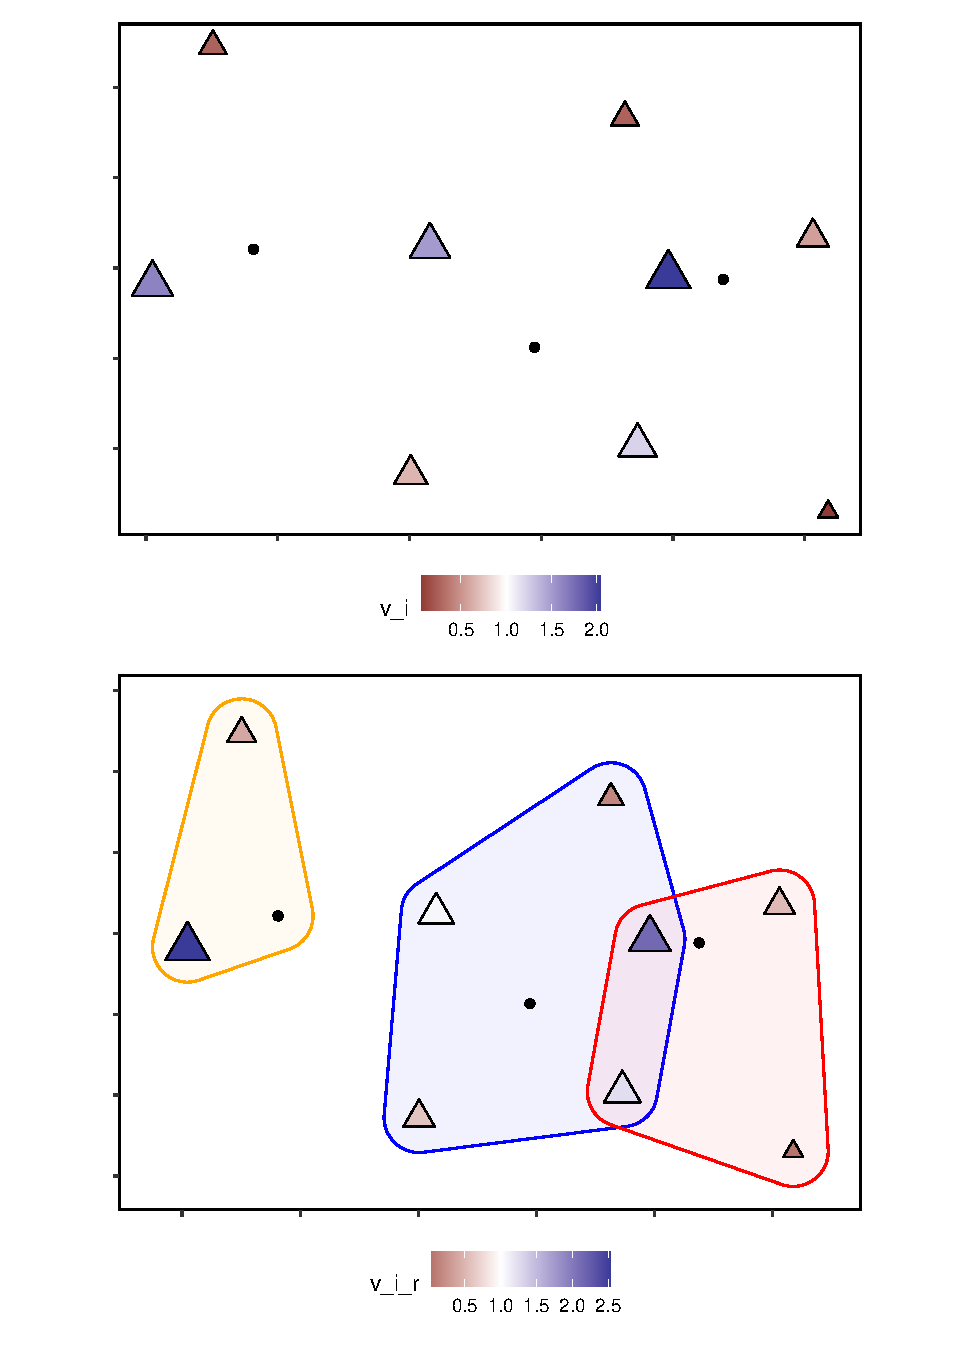
\includegraphics[width=1\linewidth]{Spatial-Availability_files/figure-latex/toy-example-availability-with-catchments-per-capita-1} \caption{\label{fig:toy-example-availability-with-catchments-per-capita}Spatial availability of jobs per capita with and without catchment restrictions }\label{fig:toy-example-availability-with-catchments-per-capita}
\end{figure}

We can see that when there are catchment restrictions population center
2, despite being relatively peripheral, has higher spatial availability
due to spatial specialization. With catchments, the spatial availability
of jobs declines from the perspective of population center 4: the
population here has skills required for jobs at a small employment
center, where they face substantial competition from other population
centers.

\hypertarget{empirical-example}{%
\section{Empirical Example}\label{empirical-example}}

Words go here.

\hypertarget{discussion}{%
\section{Discussion}\label{discussion}}

\hypertarget{comparing-accessibility-and-spatial-availability}{%
\subsection{Comparing Accessibility and Spatial
Availability}\label{comparing-accessibility-and-spatial-availability}}

Below we compare accessibility and the first case of spatial
availability illustrated above. To facilitate the comparison, we index
the measures so that the lowest value corresponds to an index of 100:

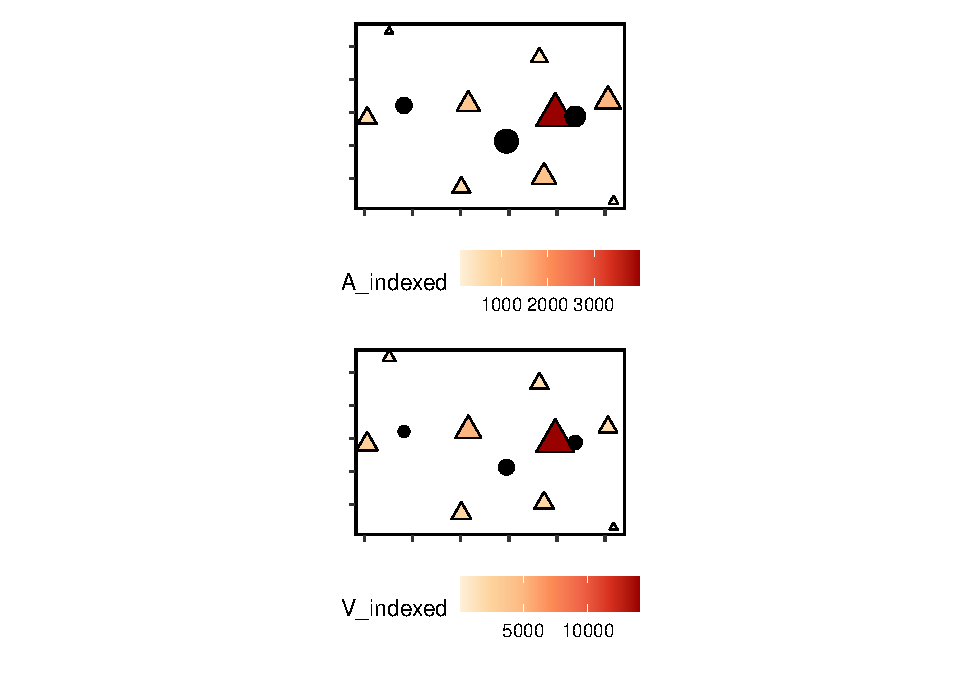
\includegraphics[width=1\linewidth]{Spatial-Availability_files/figure-latex/indexed-measures-comparison-1}

The figure suggests that high accessibility does not necessarily mean
high availability.

\hypertarget{how-are-the-these-measures-different}{%
\subsection{How are the these measures
different?}\label{how-are-the-these-measures-different}}

The sum of all spatial availability values is equal to the total number
of opportunities within the region. As such, the value for each
population center reflects how many opportunities are \emph{available}
accounting for the indivisibility of the opportunities. This provides
greater interpretability of the results. Comparatively, accessibility
values associated with each population centers reflects how many jobs
can \emph{potentially} be reached by each population center; these
values are not adjusted proportionally to the number of population
(i.e.~workers ).

Secondly, spatial availability is not robust to the modifiable unit
problem, since the estimates account for the population at the centers.
If more population centers are added, the availability adjusts
accordingly by allocating opportunities proportionally.

Further, the measure of spatial availability can be a useful way to
distinguish between high accessibility/high population centers (which
potentially can result in lower availability due to competition), and
contrariwise, low accessibility/low population centers, which may enjoy
higher availability than the accessibility calculations may suggest.
Remote, smaller population centers can be sufficiently accessible and in
close proximity to the smaller employment centers; however this
``sufficiency'' is obscured by accessibility measure by over-inflating
the accessibly of population centers which are more central to more (and
larger) employment centers. Conventional accessible does not shed light
on how sufficiently accessible opportunities are available to the
population.

As a final point, we note that the measure proposed, by producing a
concrete and interpretable number of opportunities available, can be
meaningfully compared to the total number of opportunities in the
region. Likewise for opportunities available per capita. This is an
important topic in equity analysis. For instance, considering the two
remote small population centers in the top left corner it is evident
that for individuals in population center 2, despite facing low nominal
accessibility, have a relatively high number of available jobs per
capita.

\hypertarget{conclusion}{%
\section{Conclusion}\label{conclusion}}

Words go here.

\hypertarget{references}{%
\section*{References}\label{references}}
\addcontentsline{toc}{section}{References}

\hypertarget{refs}{}
\begin{CSLReferences}{1}{0}
\leavevmode\hypertarget{ref-allen2019}{}%
Allen, J., Farber, S., 2019. A Measure of Competitive Access to
Destinations for Comparing Across Multiple Study Regions. Geographical
Analysis 52, 69--86.
doi:\href{https://doi.org/10.1111/gean.12188}{10.1111/gean.12188}

\leavevmode\hypertarget{ref-deboosere2018}{}%
Deboosere, R., El-Geneidy, A.M., Levinson, D., 2018.
Accessibility-oriented development. Journal of Transport Geography 70,
11--20.
doi:\href{https://doi.org/10.1016/j.jtrangeo.2018.05.015}{10.1016/j.jtrangeo.2018.05.015}

\leavevmode\hypertarget{ref-geurs2004}{}%
Geurs, K.T., van Wee, B., 2004. Accessibility evaluation of land-use and
transport strategies: review and research directions. Journal of
Transport Geography 12, 127--140.
doi:\href{https://doi.org/10.1016/j.jtrangeo.2003.10.005}{10.1016/j.jtrangeo.2003.10.005}

\leavevmode\hypertarget{ref-handy2020}{}%
Handy, S., 2020. Is accessibility an idea whose time has finally come?
Transportation Research Part D: Transport and Environment 83, 102319.
doi:\href{https://doi.org/10.1016/j.trd.2020.102319}{10.1016/j.trd.2020.102319}

\leavevmode\hypertarget{ref-hansen1959}{}%
Hansen, W.G., 1959. How Accessibility Shapes Land Use. Journal of the
American Institute of Planners 25, 73--76.
doi:\href{https://doi.org/10.1080/01944365908978307}{10.1080/01944365908978307}

\leavevmode\hypertarget{ref-joseph1984}{}%
Joseph, A.E., Bantock, P.R., 1984. Rural Accessibility of General
Practitioners: the Case of Bruce and Grey Counties, ONTARIO,
1901{{}}1981. The Canadian Geographer/Le Géographe canadien 28,
226--239.
doi:\href{https://doi.org/10.1111/j.1541-0064.1984.tb00788.x}{10.1111/j.1541-0064.1984.tb00788.x}

\leavevmode\hypertarget{ref-luo2003}{}%
Luo, W., Wang, F., 2003. Measures of Spatial Accessibility to Health
Care in a GIS Environment: Synthesis and a Case Study in the Chicago
Region. Environment and Planning B: Planning and Design 30, 865--884.
doi:\href{https://doi.org/10.1068/b29120}{10.1068/b29120}

\leavevmode\hypertarget{ref-miller2018}{}%
Miller, E.J., 2018. Accessibility: measurement and application in
transportation planning. Transport Reviews 38, 551--555.
doi:\href{https://doi.org/10.1080/01441647.2018.1492778}{10.1080/01441647.2018.1492778}

\leavevmode\hypertarget{ref-paez2019}{}%
Paez, A., Higgins, C.D., Vivona, S.F., 2019. Demand and level of service
inflation in Floating Catchment Area (FCA) methods. PLOS ONE 14,
e0218773.
doi:\href{https://doi.org/10.1371/journal.pone.0218773}{10.1371/journal.pone.0218773}

\leavevmode\hypertarget{ref-proffitt2017}{}%
Proffitt, D.G., Bartholomew, K., Ewing, R., Miller, H.J., 2017.
Accessibility planning in American metropolitan areas: Are we there yet?
Urban Studies 56, 167--192.
doi:\href{https://doi.org/10.1177/0042098017710122}{10.1177/0042098017710122}

\leavevmode\hypertarget{ref-shen1998}{}%
Shen, Q., 1998. Location characteristics of inner-city neighborhoods and
employment accessibility of low-wage workers. Environment and Planning
B: Planning and Design 25, 345--365.
doi:\href{https://doi.org/10.1068/b250345}{10.1068/b250345}

\leavevmode\hypertarget{ref-wilson1971}{}%
Wilson, A.G., 1971. A Family of Spatial Interaction Models, and
Associated Developments. Environment and Planning A: Economy and Space
3, 1--32. doi:\href{https://doi.org/10.1068/a030001}{10.1068/a030001}

\leavevmode\hypertarget{ref-yan2021}{}%
Yan, X., 2021. Toward Accessibility-Based Planning. Journal of the
American Planning Association 87, 409--423.
doi:\href{https://doi.org/10.1080/01944363.2020.1850321}{10.1080/01944363.2020.1850321}

\end{CSLReferences}


\end{document}
